\section{Программная реализация}

\subsection{Предобработка данных}

Прежде чем приступить к построению и обучению любой интеллектуальной системы — будь то нейронная сеть, нечеткая система или гибридный метод — критически важно убедиться в качестве и корректности входных данных. Современные алгоритмы машинного обучения крайне чувствительны к шуму, выбросам, разным масштабам признаков и пропускам, поэтому этап предобработки часто определяет успешность всей работы.

В качестве демонстрационного примера я использовал классический набор данных Iris\footnote{Fisher R.A. (1936). \emph{The use of multiple measurements in taxonomic problems}. Annals of Eugenics, 7(2):179–188.}. Этот набор содержит 150 образцов ирисов трёх видов (\emph{Iris setosa}, \emph{Versicolor}, \emph{Virginica}), описанных четырьмя числовыми признаками:
\begin{itemize}
  \item длина чашелистика (sepal length), см;
  \item ширина чашелистика (sepal width), см;
  \item длина лепестка (petal length), см;
  \item ширина лепестка (petal width), см.
\end{itemize}
Каждому образцу сопоставлен целевой класс — один из трёх видов ириса.

\medskip
\noindent\textbf{Основные этапы предобработки данных:}
\begin{enumerate}
  \item \textbf{Первичный анализ}  
    \begin{itemize}
      \item Проверка отсутствующих значений и аномалий.
      \item Вычисление базовых статистик (среднее, стандартное отклонение, квартили).
      \item Визуализация распределений (гистограммы) и парных зависимостей (scatter–matrix).
    \end{itemize}
  \item \textbf{Выявление и удаление выбросов}  
    С помощью межквартильного метода и визуальных средств (ящика с усами) отмечаются экстремальные значения, которые могут искажать обучение.
  \item \textbf{Нормализация и масштабирование}  
    Для равномерного вклада всех признаков используется стандартизация (z-score) или min–max нормализация:
    \[
      x' = \frac{x - \mu}{\sigma},\quad
      x'' = \frac{x - x_{\min}}{x_{\max}-x_{\min}}.
    \]
  \item \textbf{Разбиение на обучающую и тестовую выборки}  
    Обычно данные делятся в соотношении 70\%–30\% или 80\%–20\%, с последующим стратифицированным отбором образцов, чтобы сохранить пропорции классов.
\end{enumerate}

\subsection{Инструменты анализа}

Для качественной предобработки и первичной оценки данных используются следующие ключевые приёмы визуализации:

\begin{description}
  \item[Гистограмма (Histogram)]  
    \hfill 
    \begin{itemize}
      \item \textbf{Назначение:} 
        
        оценить форму распределения одного числового признака, выявить асимметрию, мультимодальность и выбросы.
      \item \textbf{Как читать:} 
        
        по горизонтали — интервалы значений (бины), по вертикали — количество образцов.  
      \item \textbf{Рекомендации:}  
        \begin{itemize}
          \item Подберите число бинов так, чтобы не терялось основное «полотно» распределения, но и не было слишком «рвано».  
          \item Обратите внимание на пики — возможные подгруппы данных.  
          \item Узкие «хвосты» помогут заметить редкие выбросы.
        \end{itemize} 
    \end{itemize}

  \item[Boxplot–диаграмма (Box–Whisker)]  
    \hfill
    \begin{itemize}
      \item \textbf{Назначение:} 
        
        сравнить распределения одного признака между группами (видами iris), одновременно увидеть медиану, квартильные границы и выбросы.
      \item \textbf{Как читать:}  
        \begin{itemize}
          \item Ящик (box) — межквартильный интервал (Q1–Q3), линия внутри — медиана.  
          \item Усы (whiskers) — выборочные границы (обычно Q1−-1.5 \cdot IQR, Q3+1.5 \cdot IQR).  
          \item Точки за усами — выбросы.
        \end{itemize}
      \item \textbf{Рекомендации:}  
        \begin{itemize}
          \item Сравнивайте положения медиан для разных групп.  
          \item Используйте одну палитру для согласованности.  
          \item При разметке терминов в нечеткой системе берите Q1, Q2, Q3 как опорные точки.
        \end{itemize}
    \end{itemize}

  \item[Матрица рассеяния (Scatter–matrix)]  
    \hfill
    \begin{itemize}
      \item \textbf{Назначение:} 
        
        одновременно визуализировать попарные зависимости и распределения всех признаков.
      \item \textbf{Как читать:}  
        \begin{itemize}
          \item Диагональные ячейки — гистограммы каждого признака.  
          \item Вне диагонали — точечные диаграммы (scatter plots) для пары признаков.
        \end{itemize}
      \item \textbf{Рекомендации:}  
        \begin{itemize}
          \item Ищите пары с минимальным перекрытием классов — эти сочетания наиболее информативны для классификатора.  
          \item Линейная или кластераная структура подскажет, что выбирать в качестве antecedent–признаков.
        \end{itemize}
    \end{itemize}

  \item[K–Means кластеризация (Cluster Plot)]  
    \hfill
    \begin{itemize}
      \item \textbf{Назначение:} быстро оценить естественную группировку данных в выбранном признаковом пространстве.
      \item \textbf{Как читать:}  
        \begin{itemize}
          \item Точки раскрашены по присвоенному кластеру.  
          \item Центроиды отображаются метками (крестиками).  
          \item Легенда и подписи кластеров помогают связать группы с реальными классами.
        \end{itemize}
      \item \textbf{Рекомендации:}  
        \begin{itemize}
          \item Используйте кластер-плот для предпосева числа терминов в нечеткой системе.  
          \item Оценивайте степень «смешивания» точек разных классов внутри одного кластера.  
          \item Корректируйте число кластеров ($k$) и наблюдайте устойчивость центроидов.
        \end{itemize}
    \end{itemize}
\end{description}

\subsection{Анализ исходных данных (Iris Dataset)}


Прежде чем приступать к построению нечеткой сети, необходимо тщательно изучить и подготовить исходный датасет. В качестве демонстрационного примера мы используем классический набор \emph{Iris} (150 образцов, 4 числовых признака, 3 класса).

\subsubsection{Статистическое описание}
\begin{table}[H]
  \centering
  \caption{Базовые статистические характеристики признаков Iris Dataset.}
  \begin{tabular}{lrrrr}
    \toprule
    Признак & Среднее & СКО & Мин. & Макс. \\
    \midrule
    sepal length (cm) & 5.84 & 0.83 & 4.30 & 7.90 \\
    sepal width  (cm) & 3.06 & 0.44 & 2.00 & 4.40 \\
    petal length (cm) & 3.76 & 1.77 & 1.00 & 6.90 \\
    petal width  (cm) & 1.20 & 0.76 & 0.10 & 2.50 \\
    \bottomrule
  \end{tabular}
  \label{tab:iris_stats}
\end{table}

\subsubsection{Распределение признаков}

На рис.~\ref{fig:iris_histos} представлены гистограммы всех четырёх признаков, построенные с цветовой палитрой.
\begin{figure}[H]
  \centering
  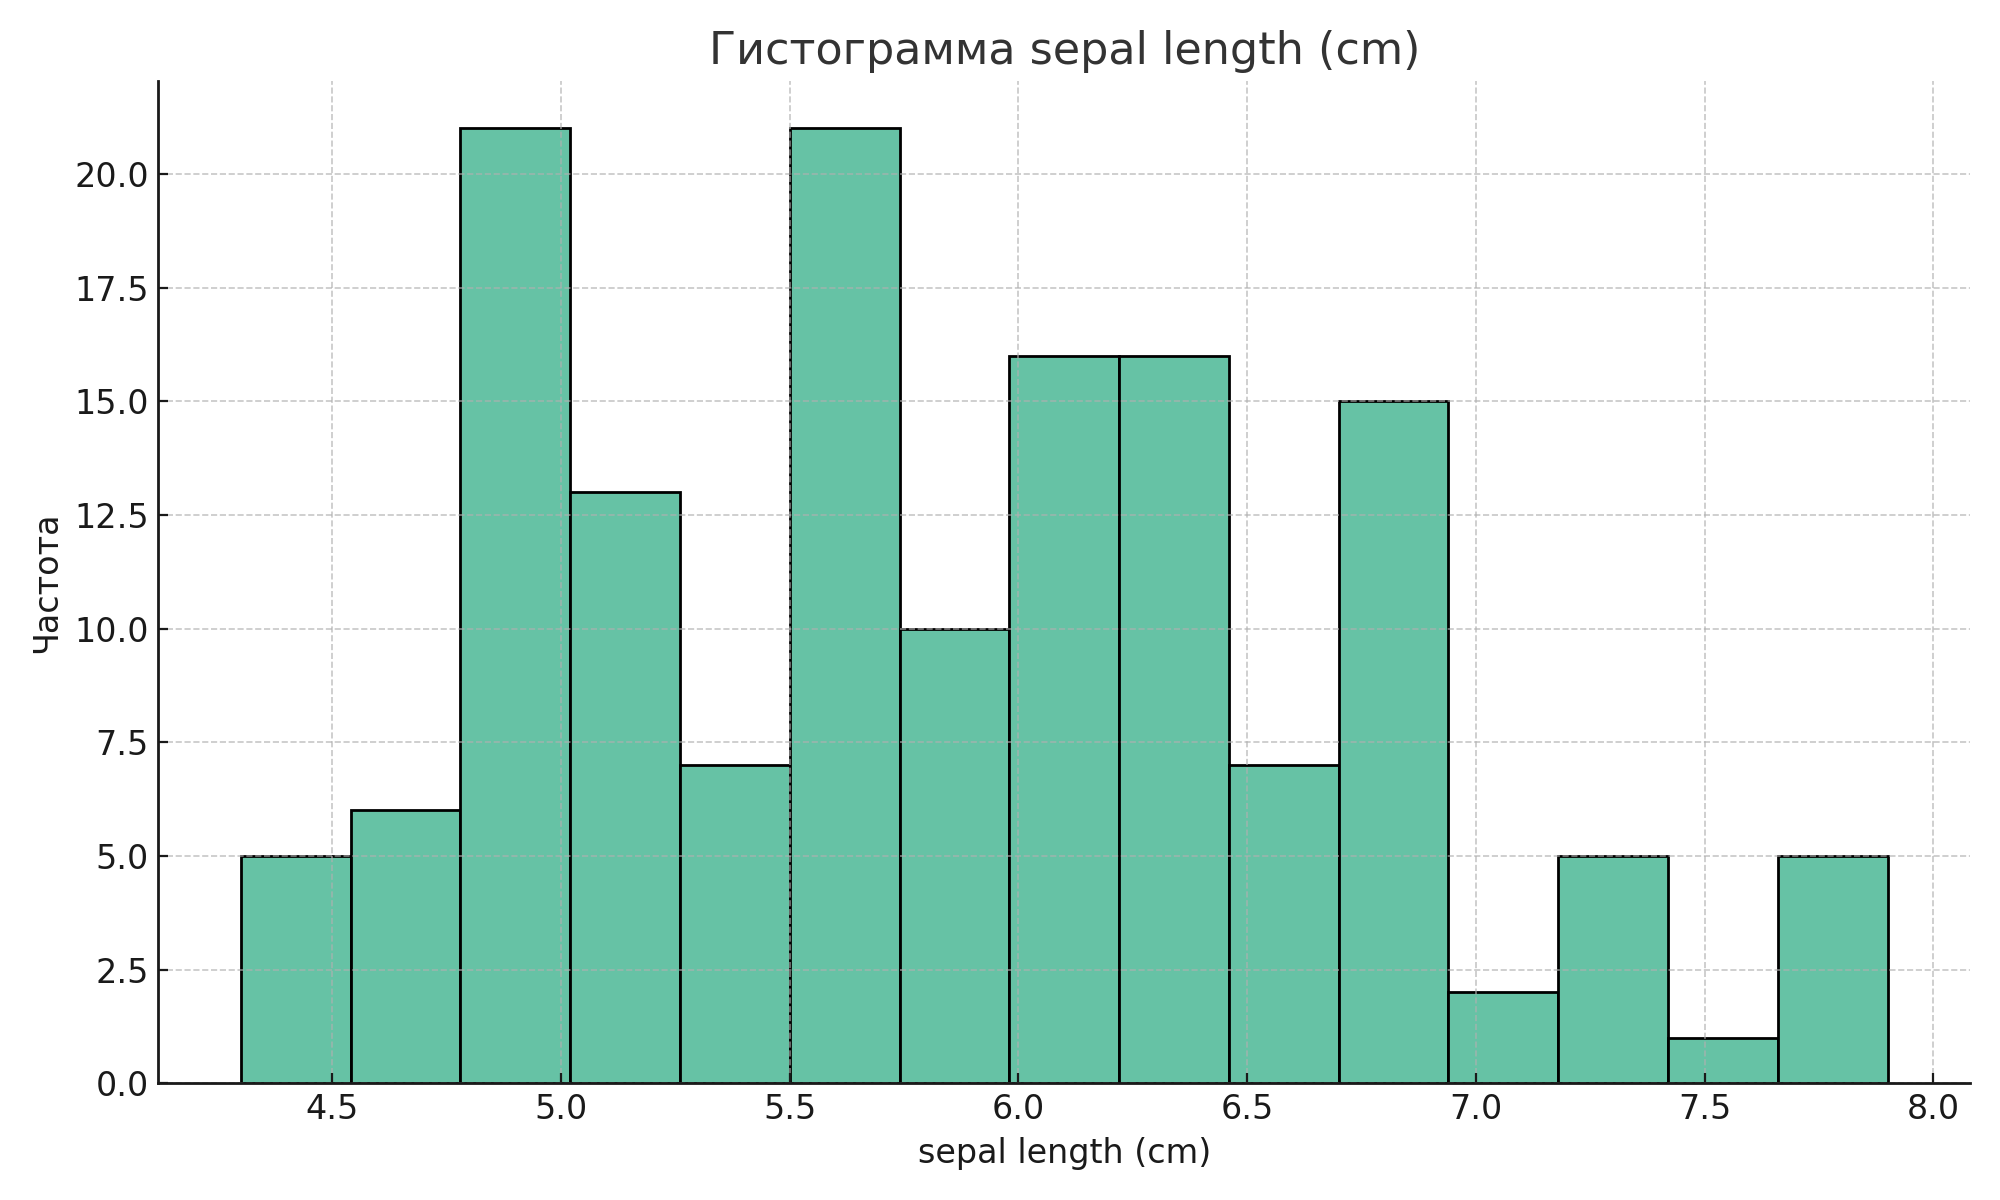
\includegraphics[width=0.8\textwidth]{images/histo_sepal_length_cm_cb2.png}\\[6pt]
  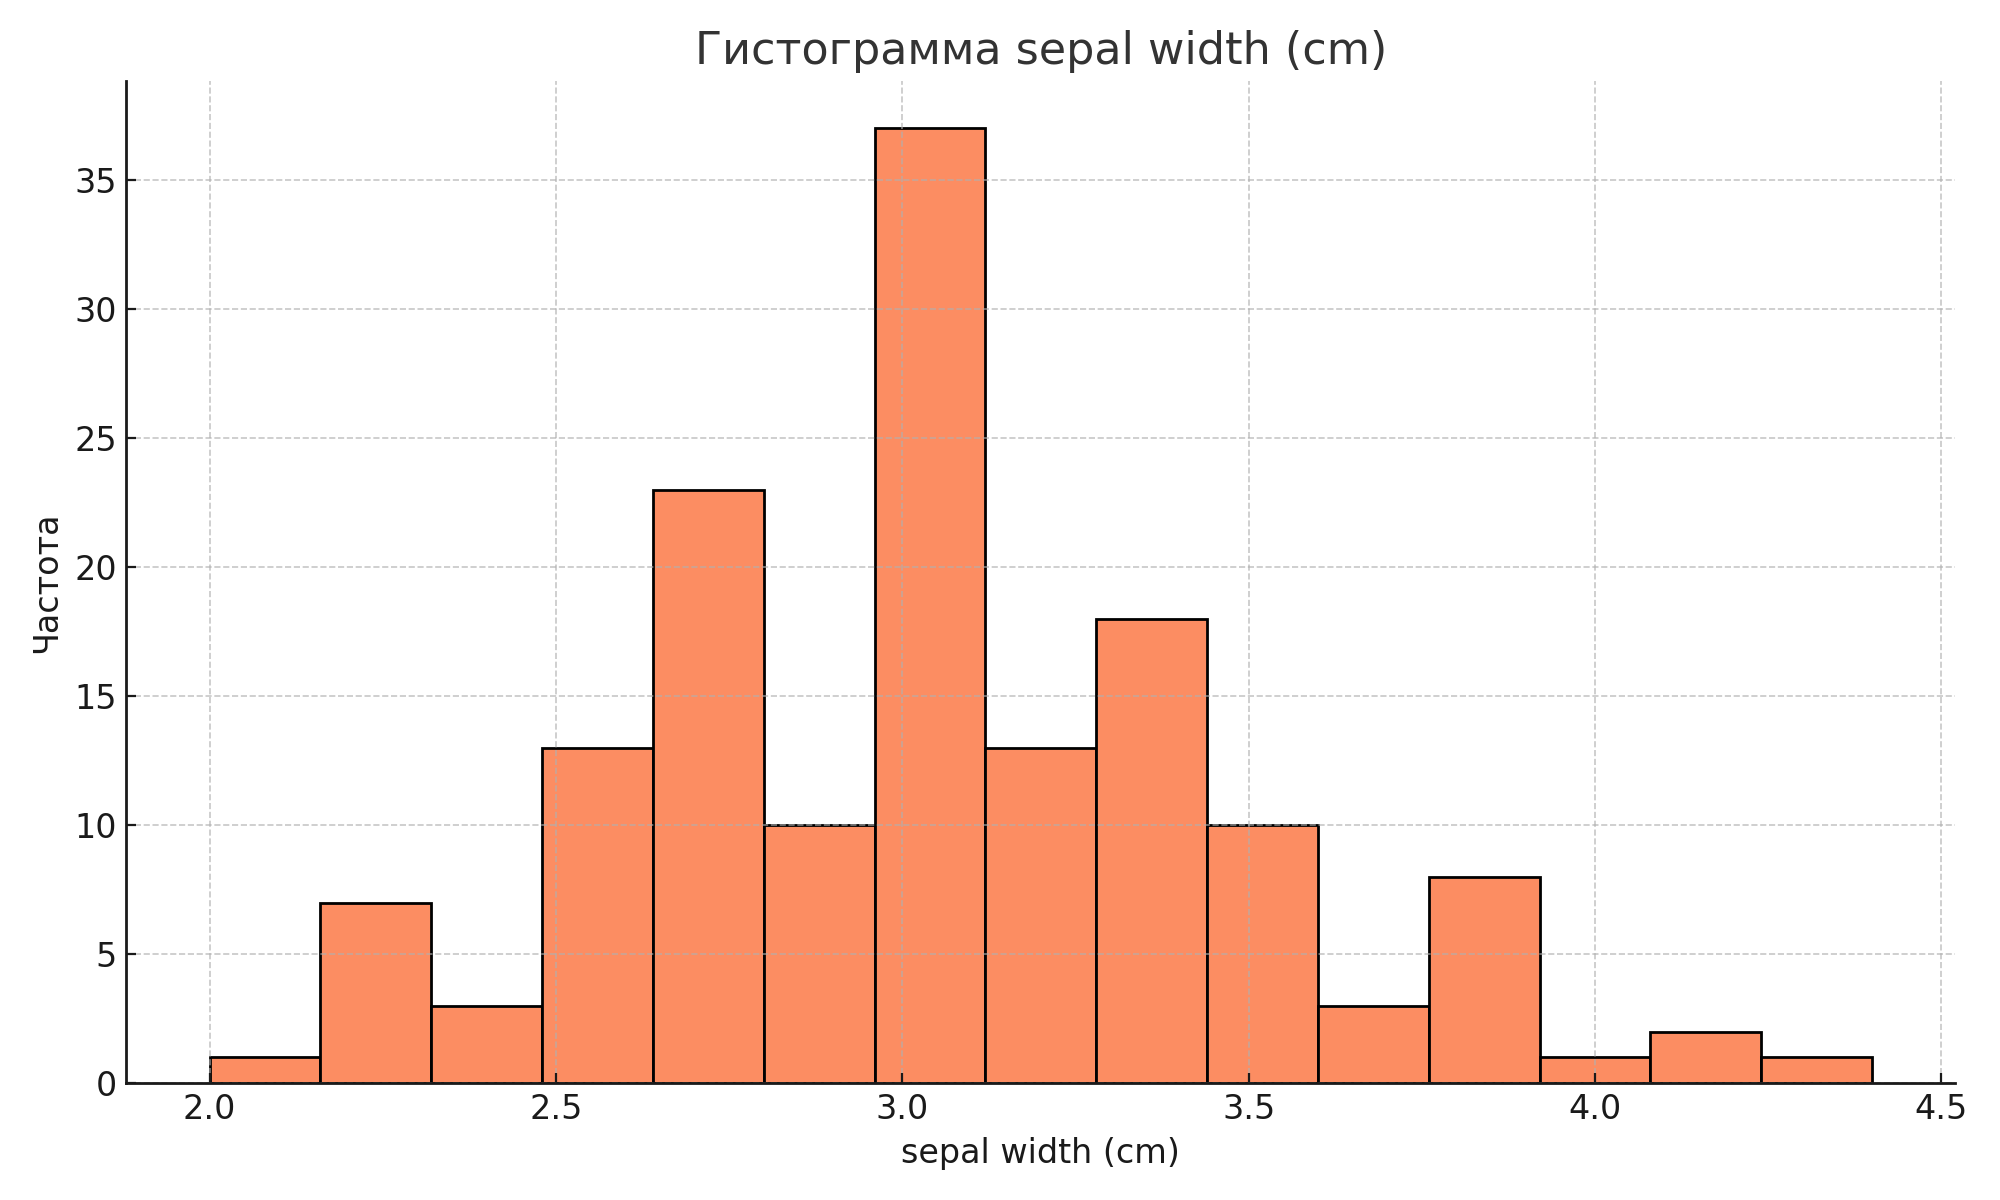
\includegraphics[width=0.8\textwidth]{images/histo_sepal_width_cm_cb2.png}
  \caption{Гистограммы распределений признаков Iris Dataset.}
  \label{fig:iris_histos}
\end{figure}

\begin{figure}[H]\ContinuedFloat
  \centering
  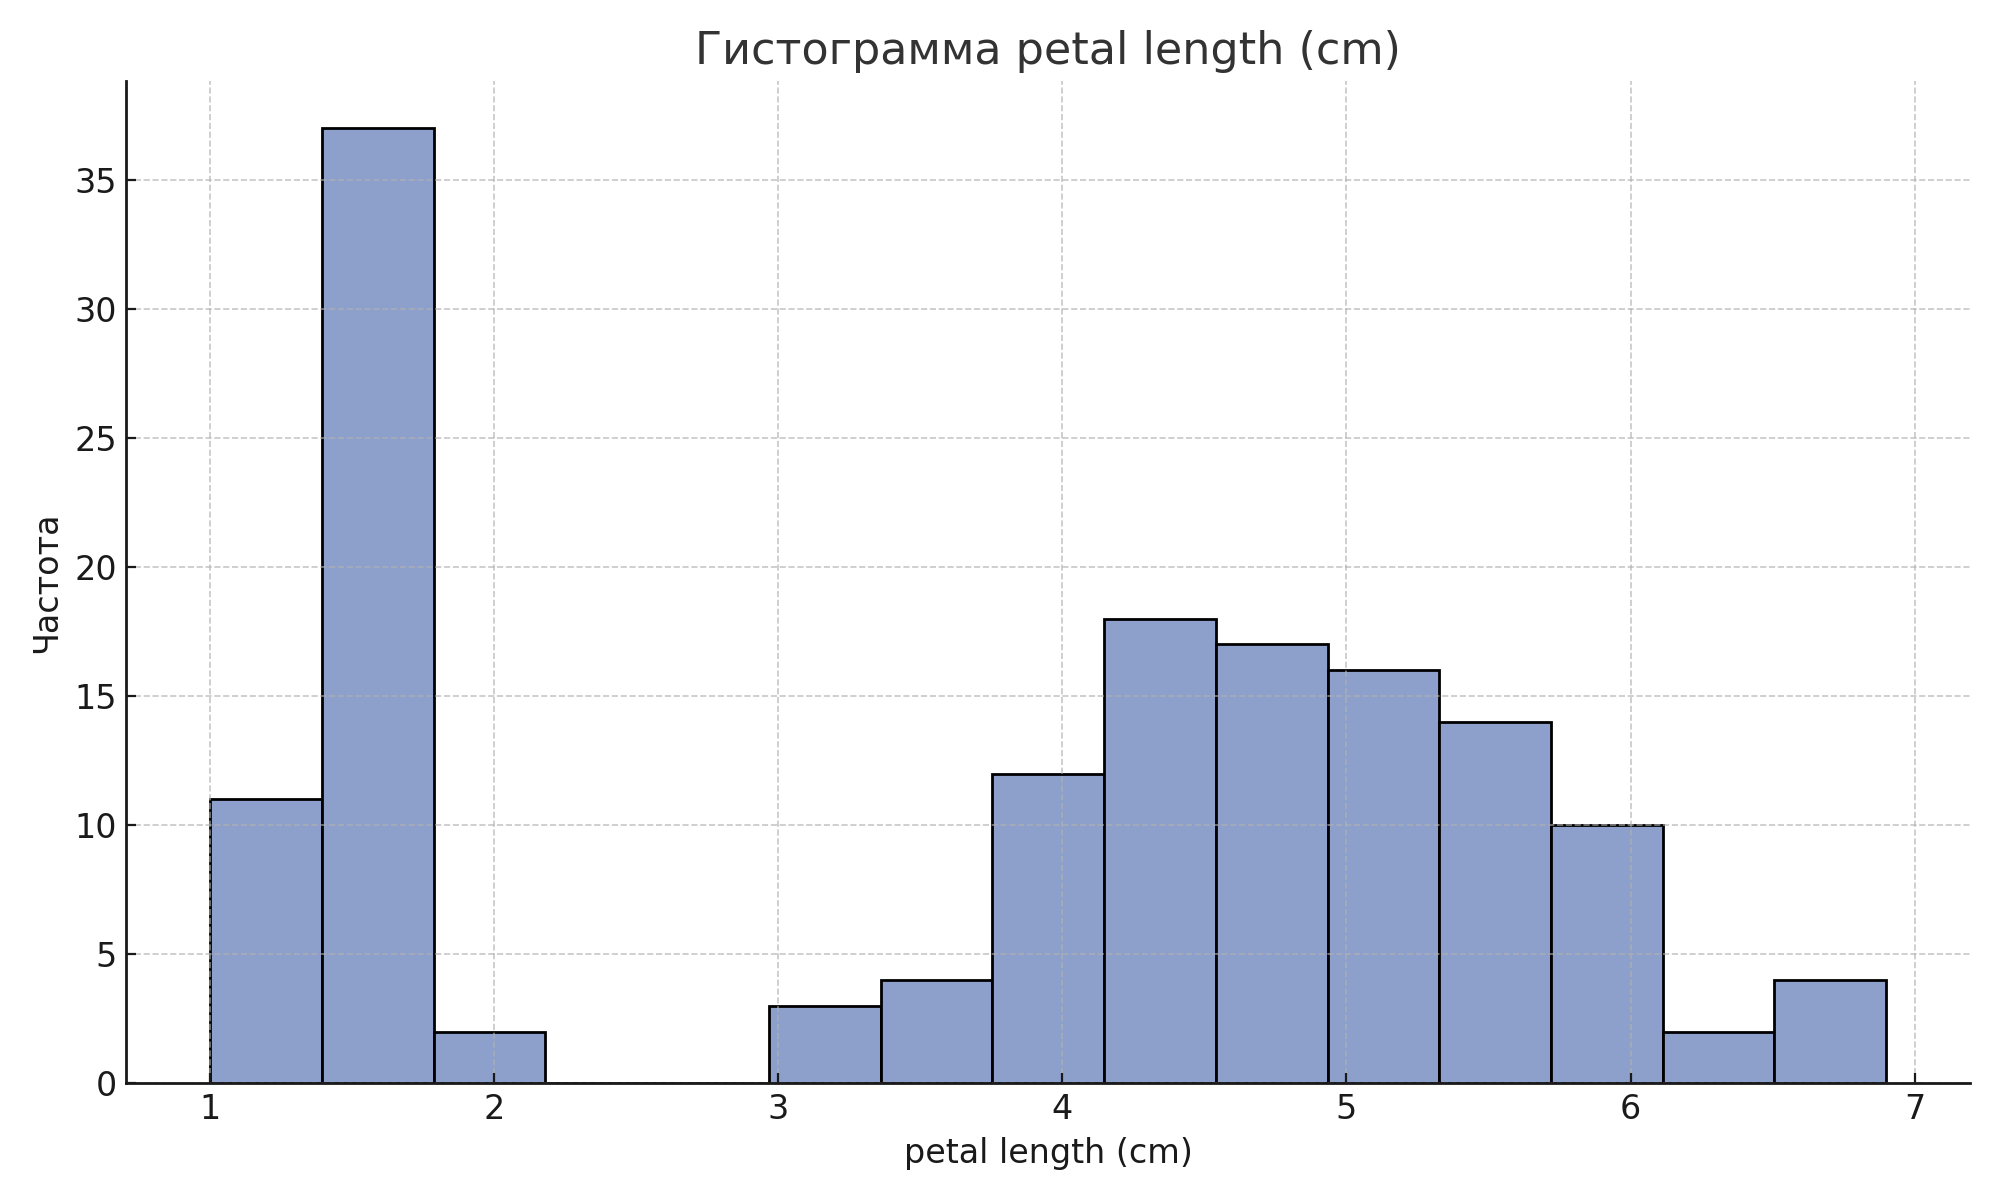
\includegraphics[width=0.8\textwidth]{images/histo_petal_length_cm_cb2.png}\\[6pt]
  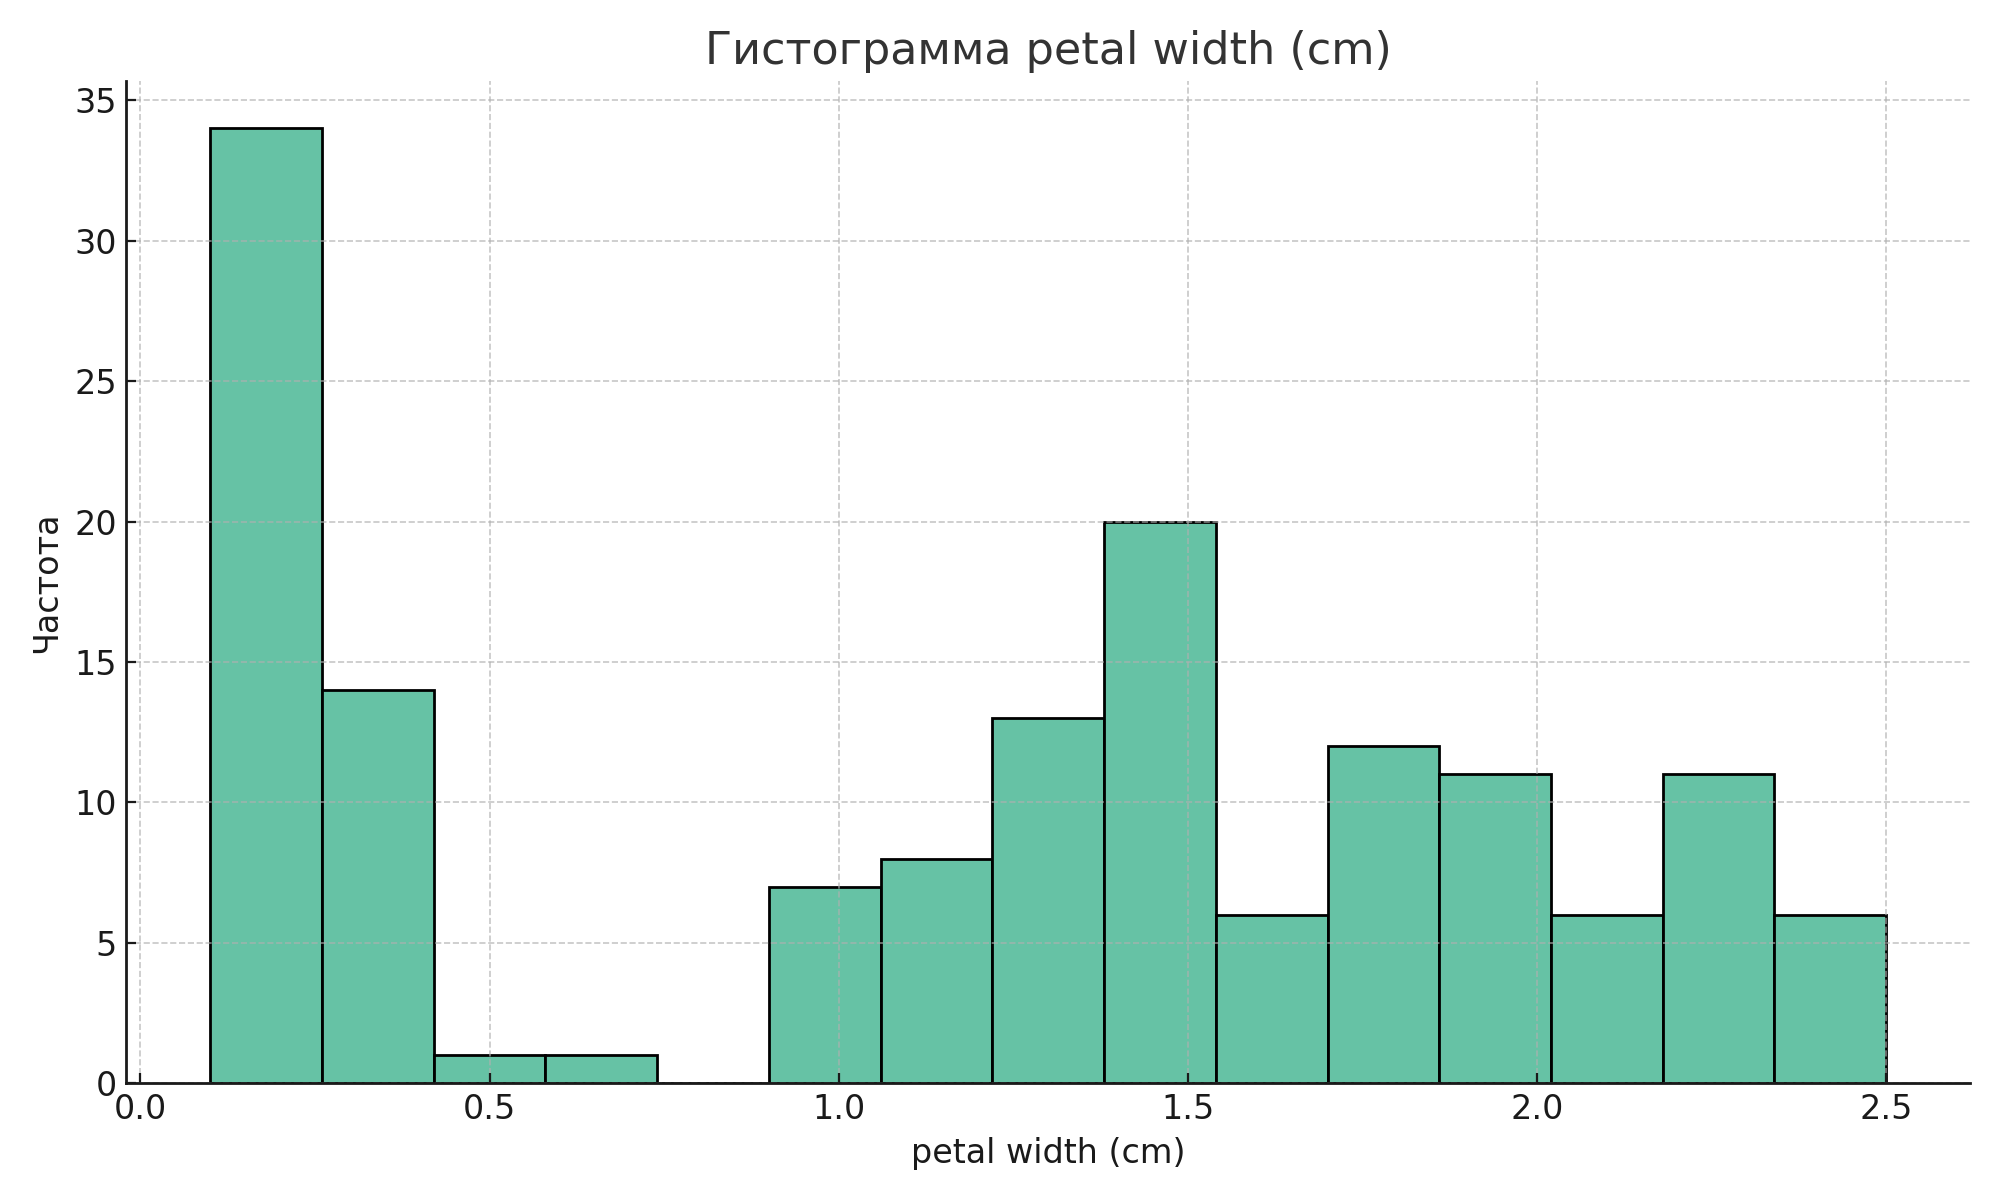
\includegraphics[width=0.8\textwidth]{images/histo_petal_width_cm_cb2.png}
  % не вызываем \caption — подпись продолжится от предыдущего блока
\end{figure}

\paragraph{Выводы.}
\begin{itemize}
  \item \textbf{sepal length} демонстрирует почти нормальное распределение с лёгкой дву­пиковостью (Setosa vs.~остальные виды).
  \item \textbf{sepal width} скошено вправо, большинство значений в [2.5, 3.5] см.
  \item \textbf{petal length} и \textbf{petal width} отчётливо мультимодальны: Setosa образует узкий «низ» (1–2 см), Versicolor и Virginica смещены вправо.
\end{itemize}

\subsubsection{Boxplot–анализ по видам}

Распределения по классам показаны на рис.~\ref{fig:iris_boxplots_vertical}.
\begin{figure}[H]
  \centering
  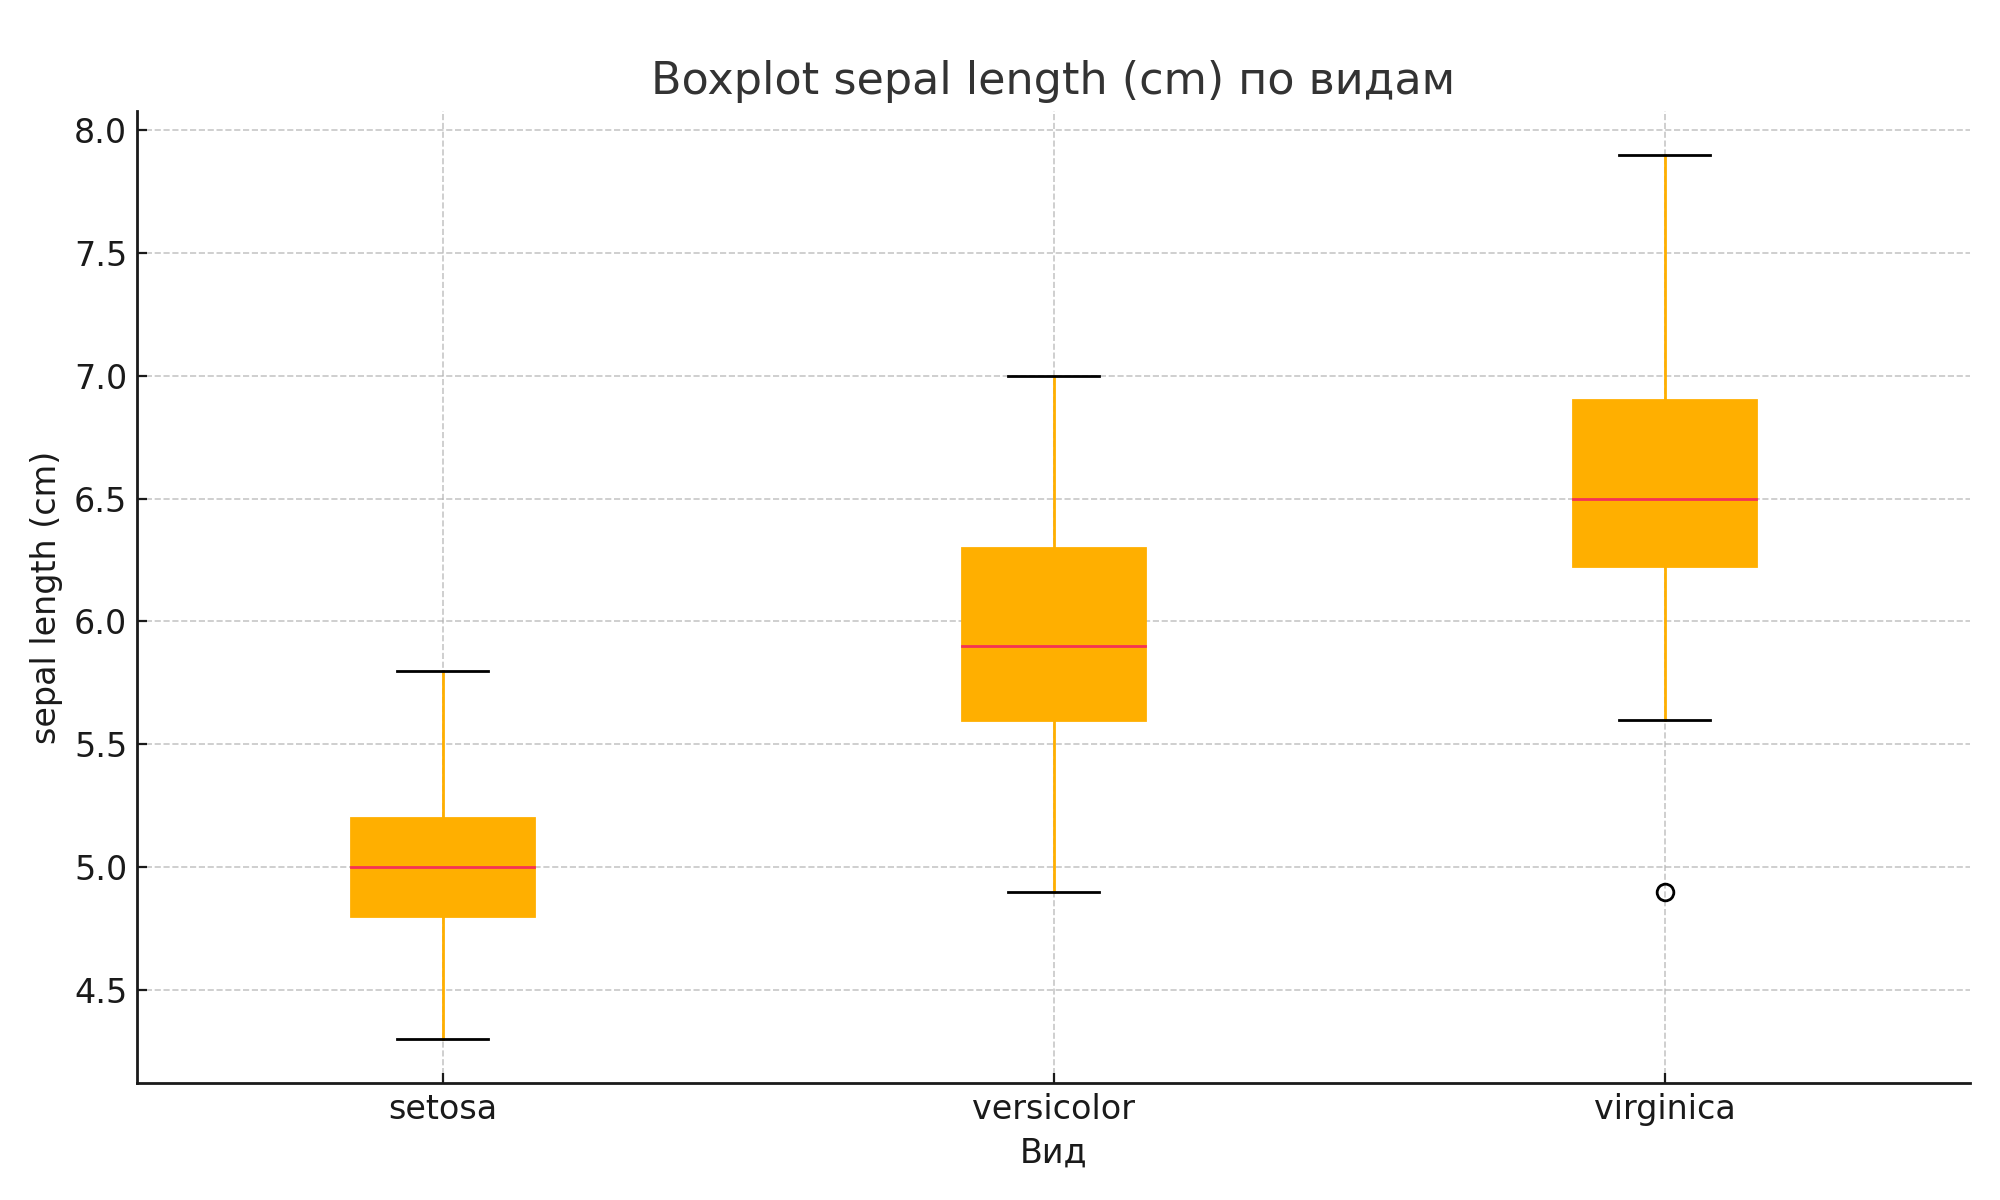
\includegraphics[width=0.8\textwidth]{images/box_sepal_length_cm_cb2.png}\\[6pt]
  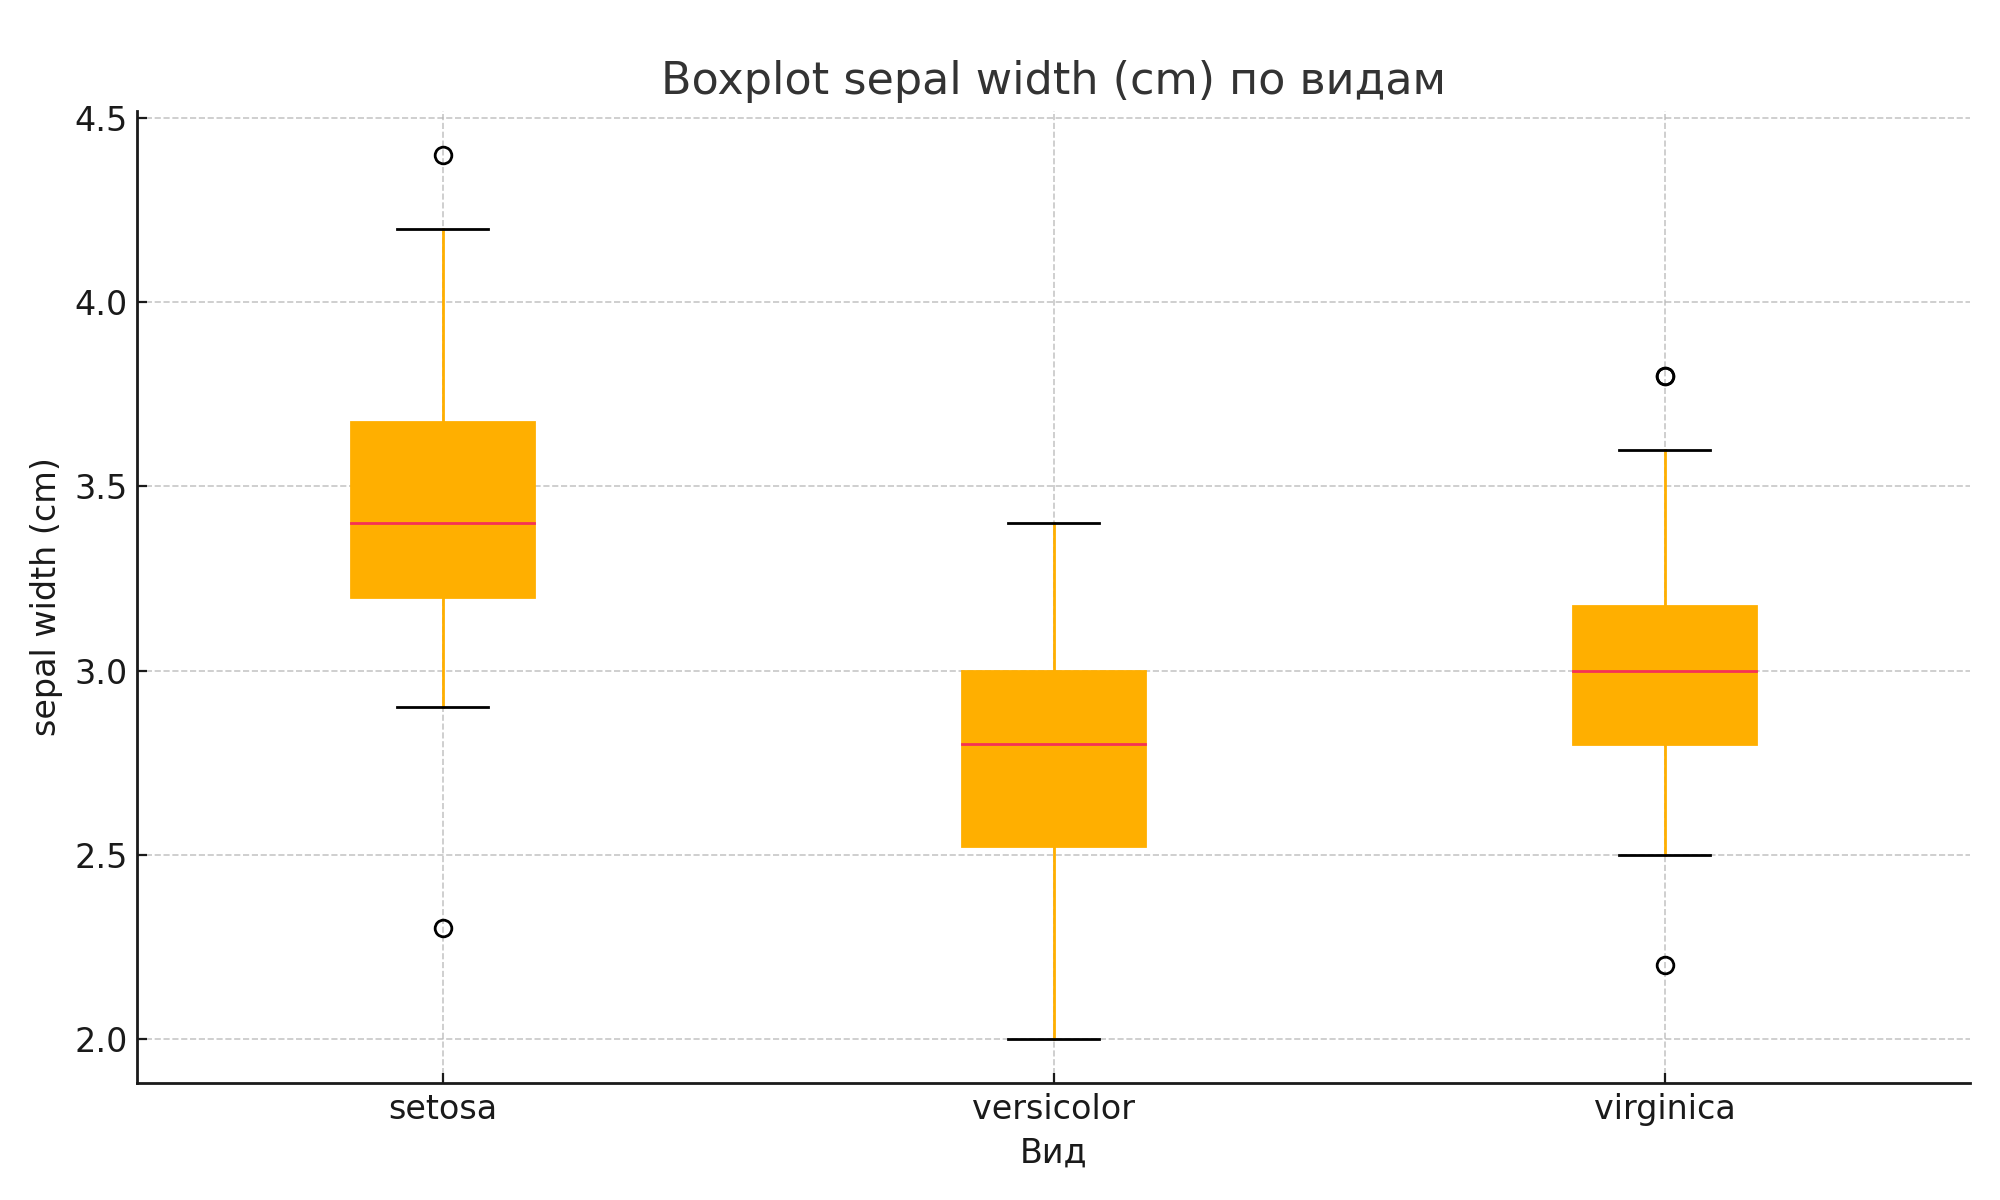
\includegraphics[width=0.8\textwidth]{images/box_sepal_width_cm_cb2.png}
  \caption{Boxplot–диаграммы признаков по видам Iris Dataset.}
  \label{fig:iris_boxplots_vertical}
\end{figure}

\begin{figure}[H]
  \ContinuedFloat
  \centering
  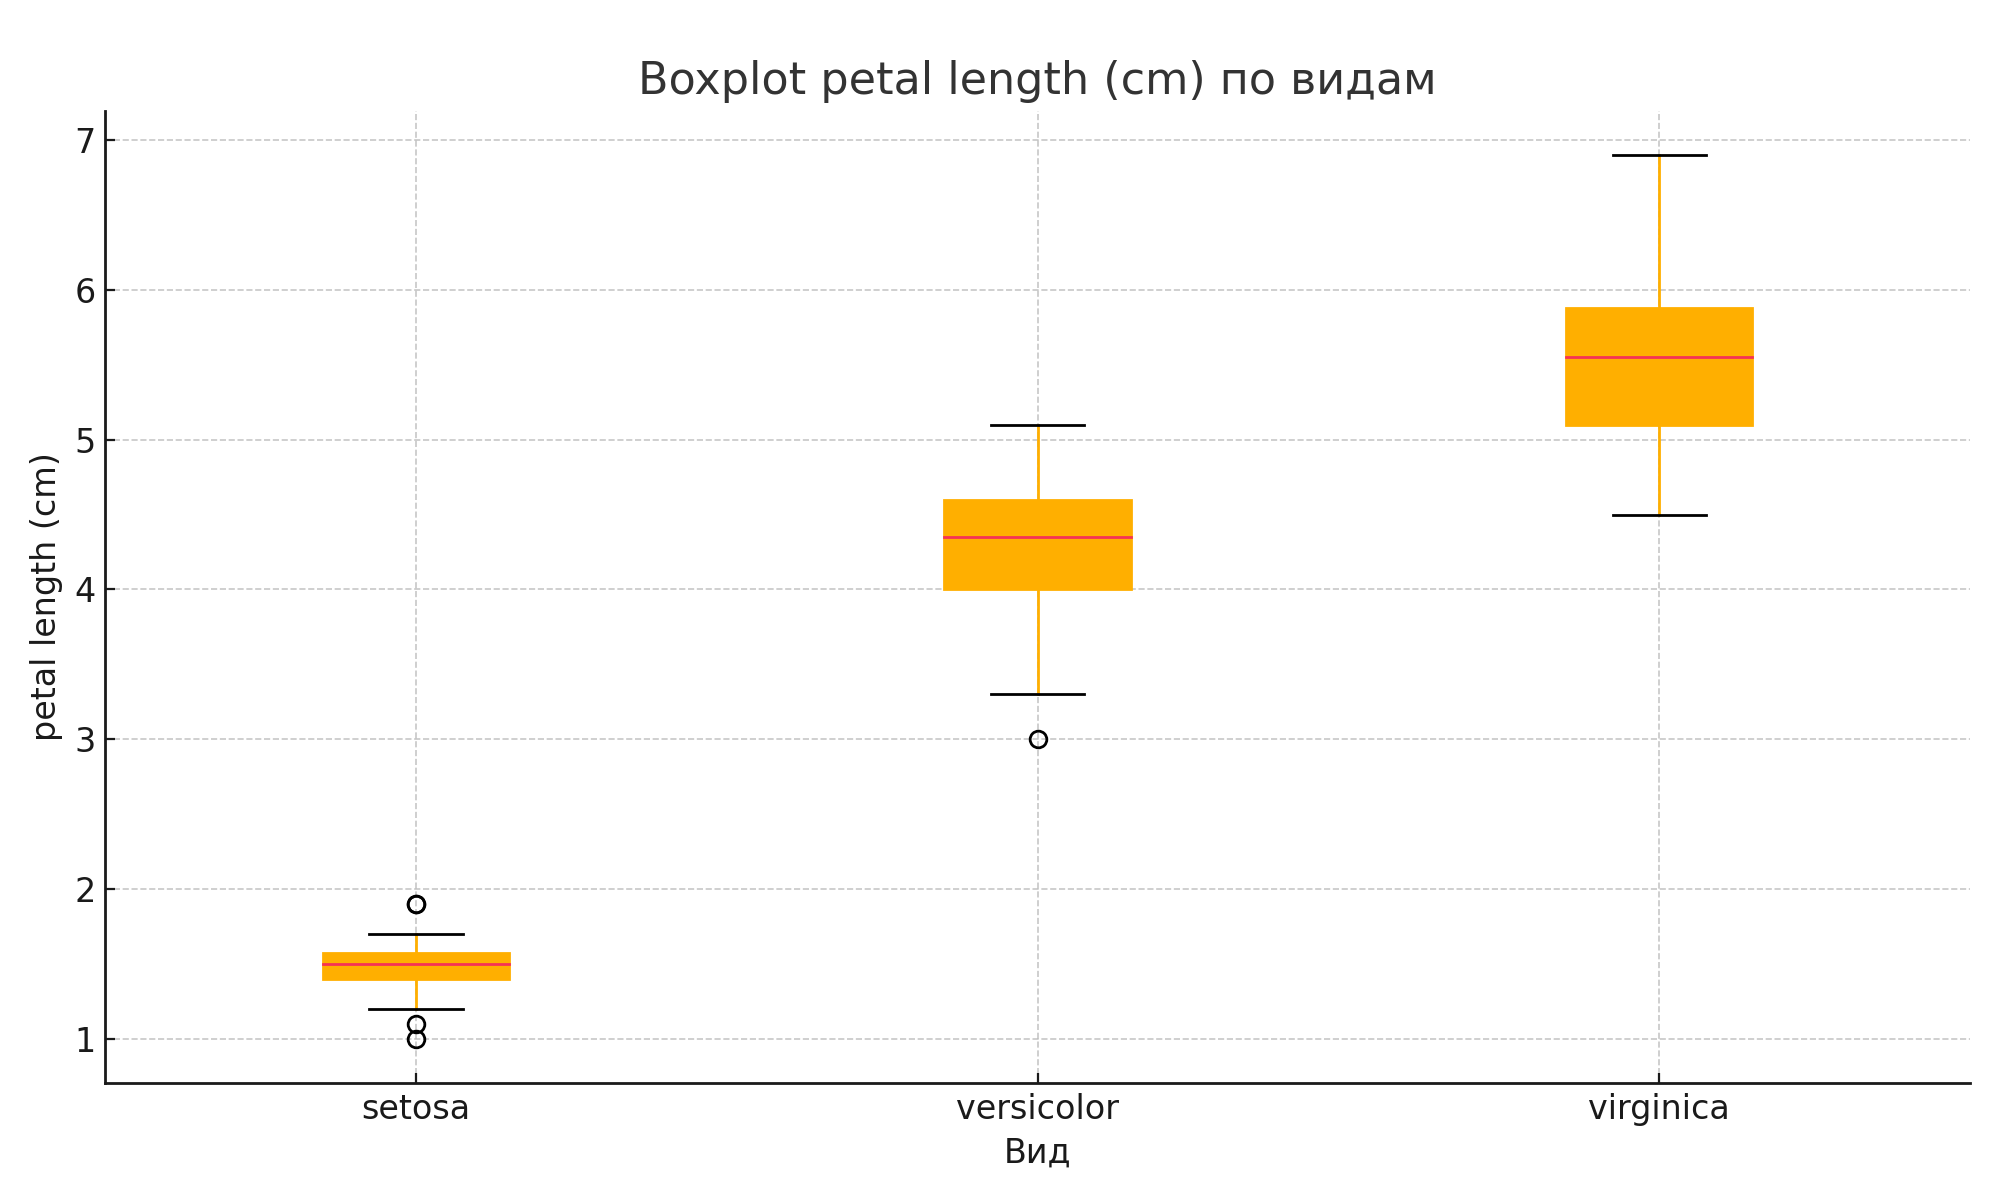
\includegraphics[width=0.8\textwidth]{images/box_petal_length_cm_cb2.png}\\[6pt]
  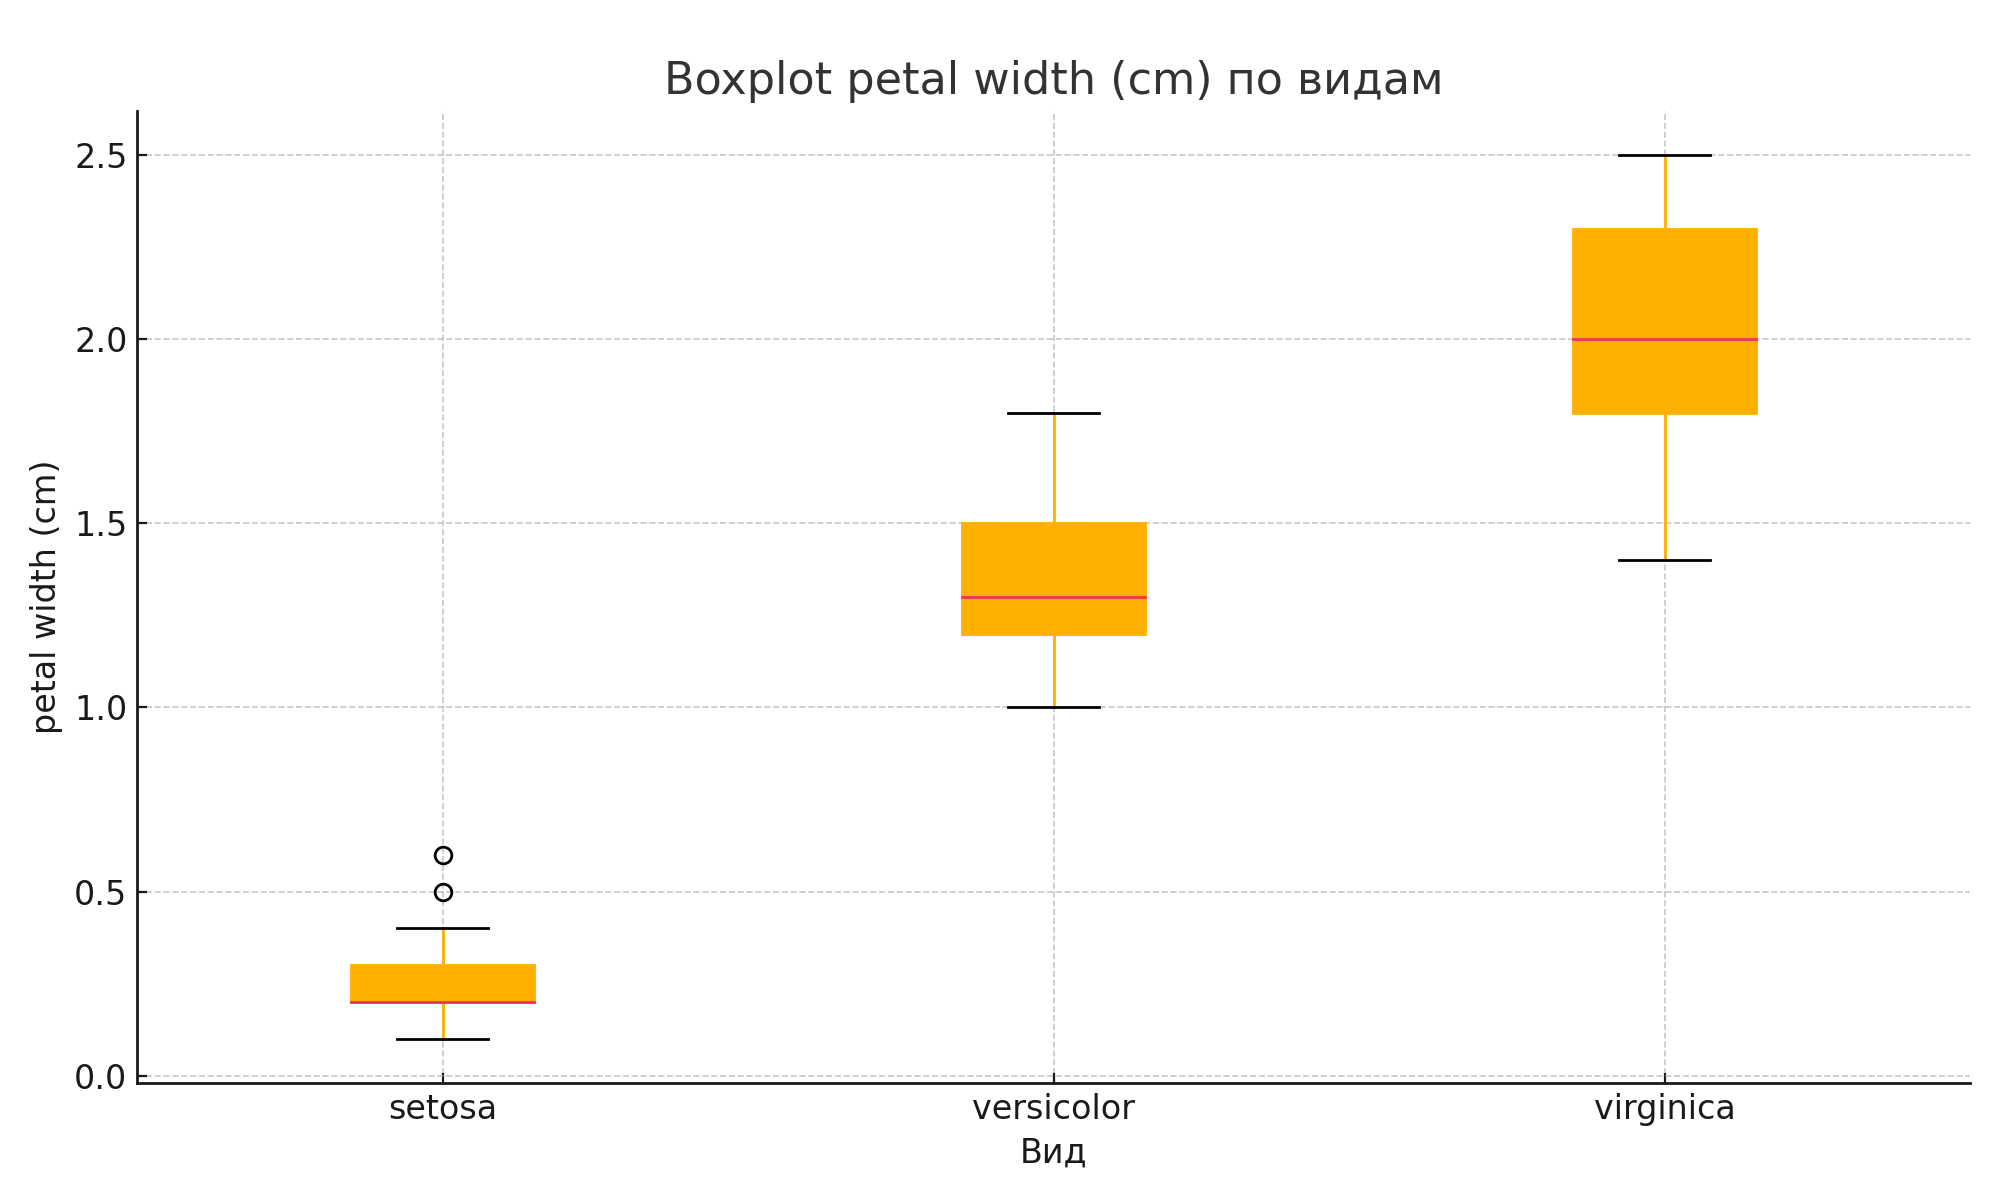
\includegraphics[width=0.8\textwidth]{images/box_petal_width_cm_cb2.png}
  \caption{Boxplot–диаграммы признаков по видам Iris Dataset.}
\end{figure}

\paragraph{Выводы.}
\begin{itemize}
  \item Для \emph{petal length/width} квартильные интервалы видов не перекрываются → признаки почти идеальны для классификации.
  \item Для \emph{sepal length/width} наблюдаются пересечения квартилей Versicolor и Virginica, поэтому они менее информативны в отрыве от лепестковых.
\end{itemize}

\subsubsection{Парная визуализация (Scatter–matrix)}

На рис.~\ref{fig:scatter_matrix} приведена матрица рассеяния всех пар признаков.

\begin{figure}[ht]
  \centering
  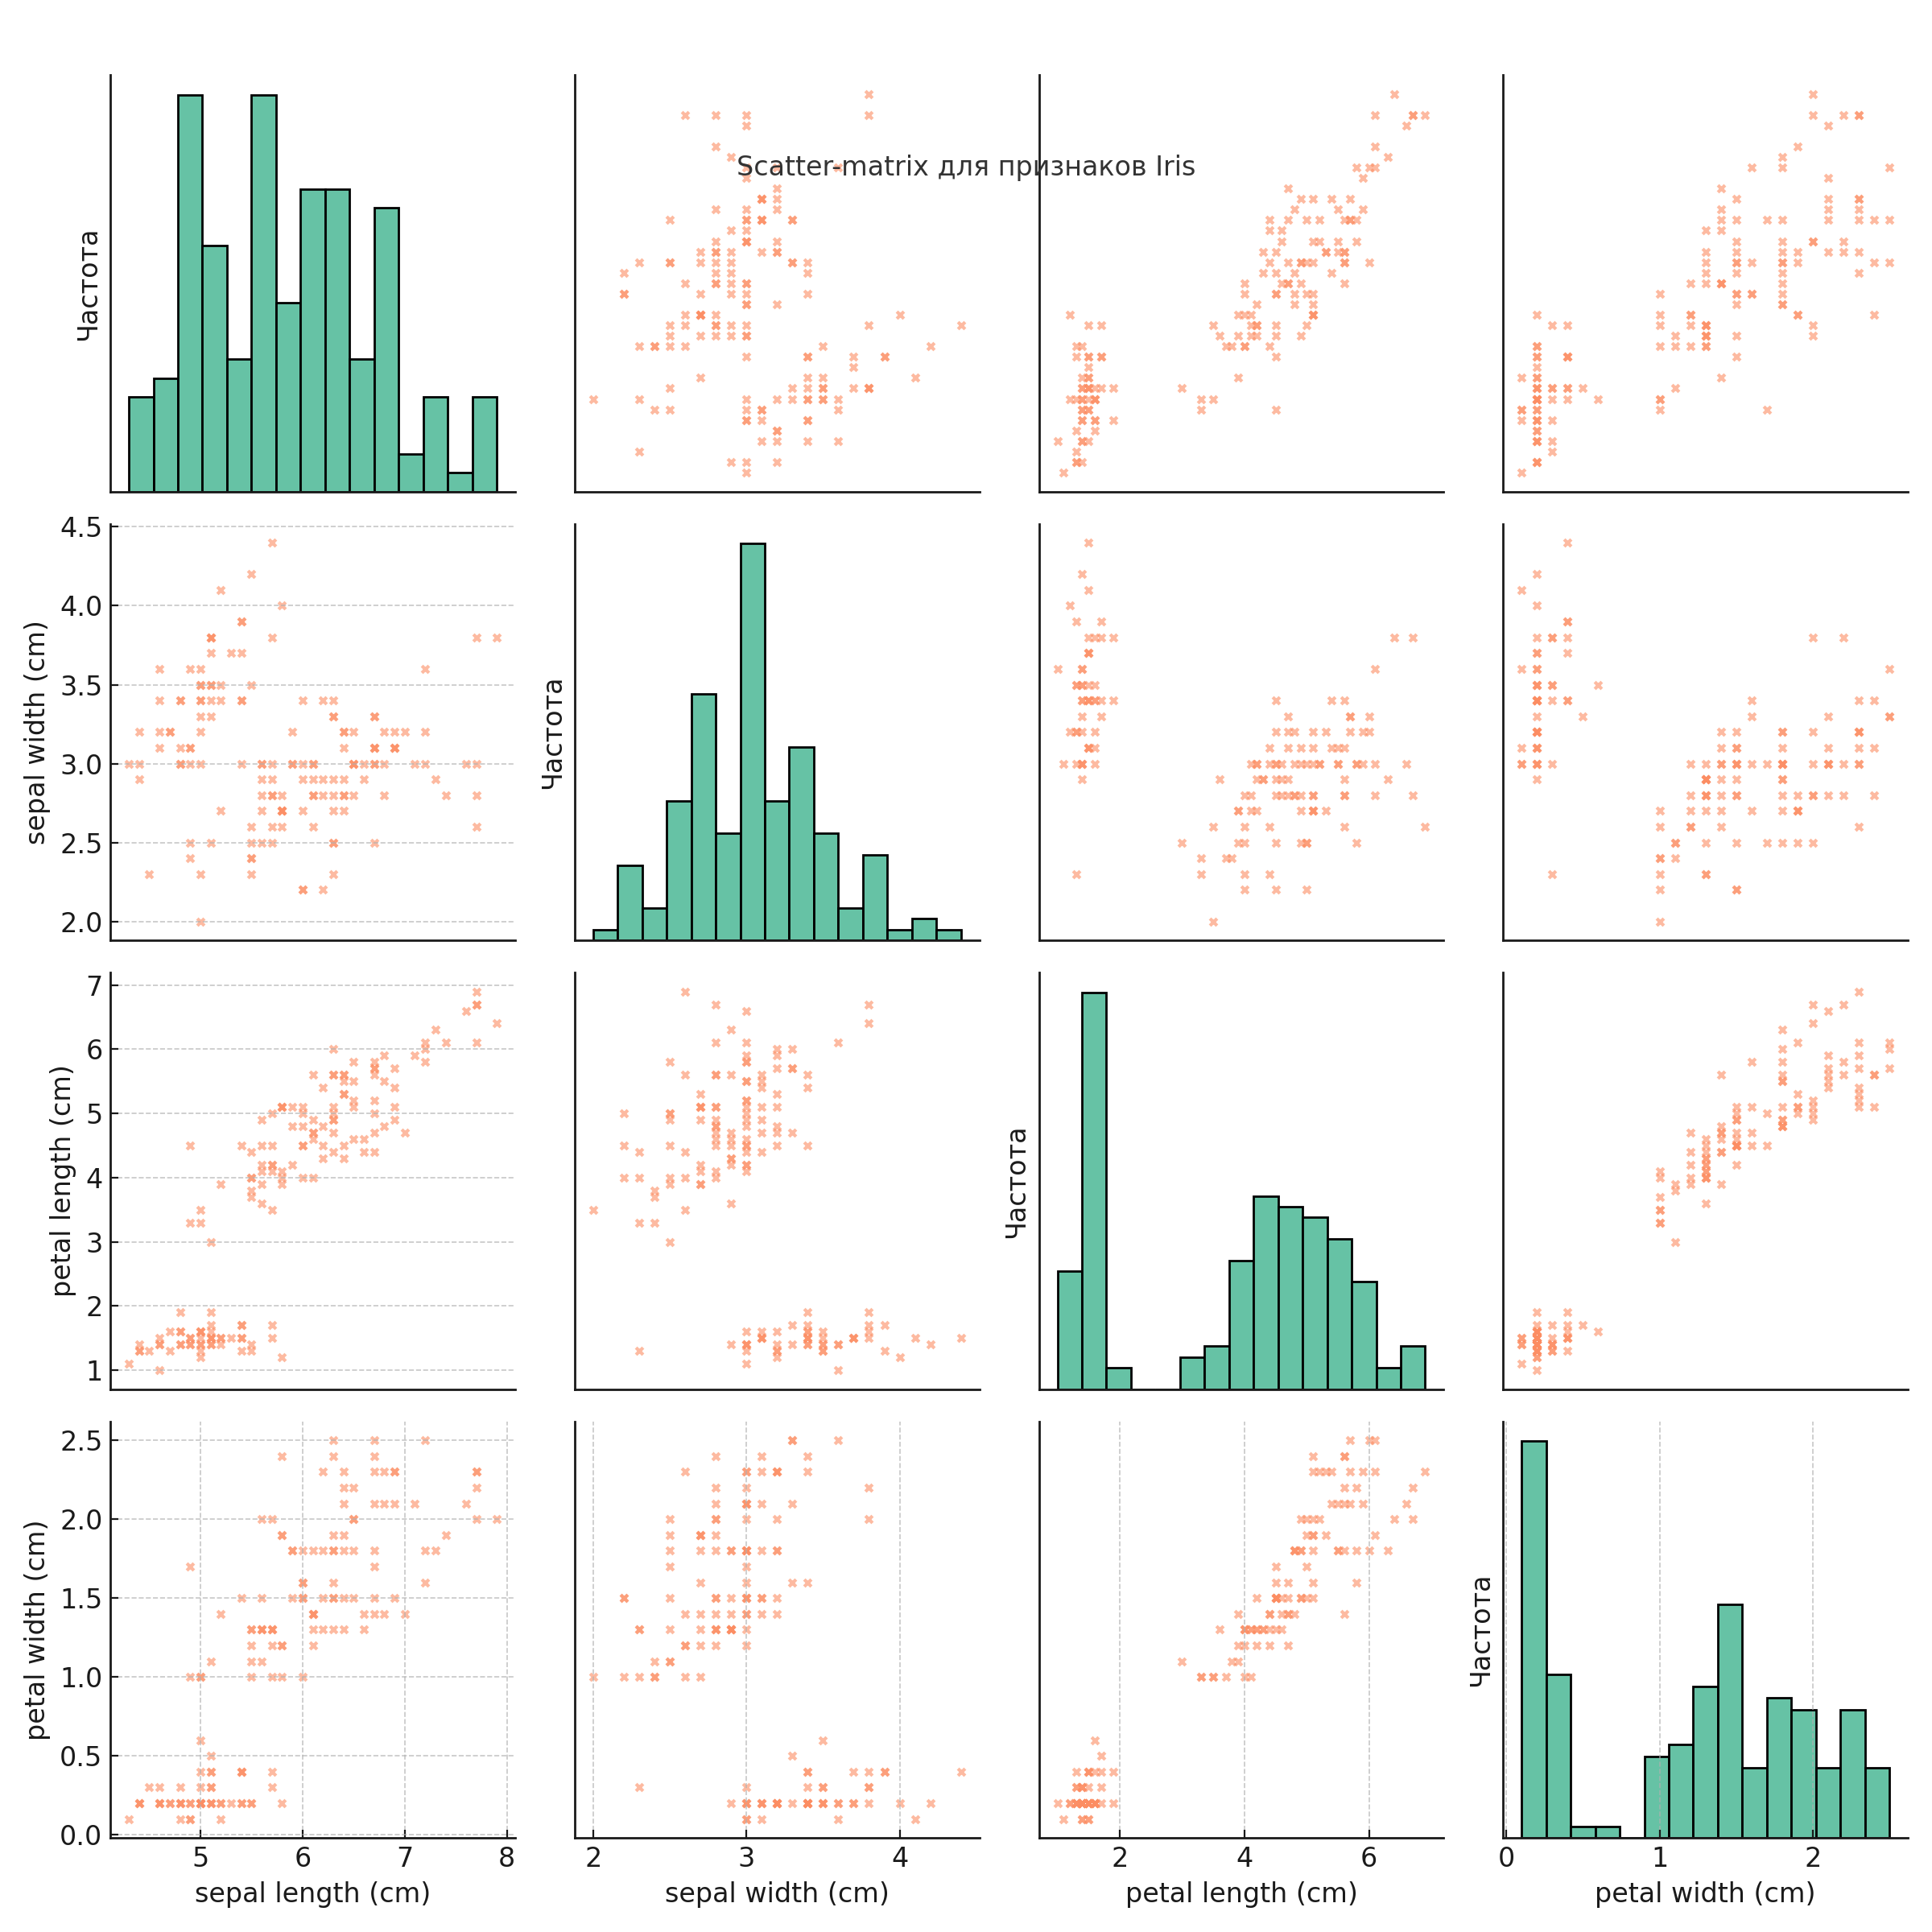
\includegraphics[width=\textwidth]{images/scatter_matrix_cb2.png}
  \caption{Scatter–matrix для признаков Iris.}
  \label{fig:scatter_matrix}
\end{figure}

\paragraph{Выводы.}
\begin{itemize}
  \item Самая сильная корреляция между \emph{petal length} и \emph{petal width}.
  \item Комбинации (\emph{sepal length}, \emph{petal length}) и (\emph{petal length}, \emph{petal width}) дают линейно разделимые классы.
  \item Пара (\emph{sepal width}, \emph{sepal length}) менее информативна.
\end{itemize}

\subsubsection{Кластеризация K–Means}

Наконец, на рис.~\ref{fig:kmeans_cb2} представлена K–Means кластеризация ($k=3$) по паре (\emph{sepal length}, \emph{petal length}), использующая ту же палитру ColorBrewer\_2.

\begin{figure}[ht]
  \centering
  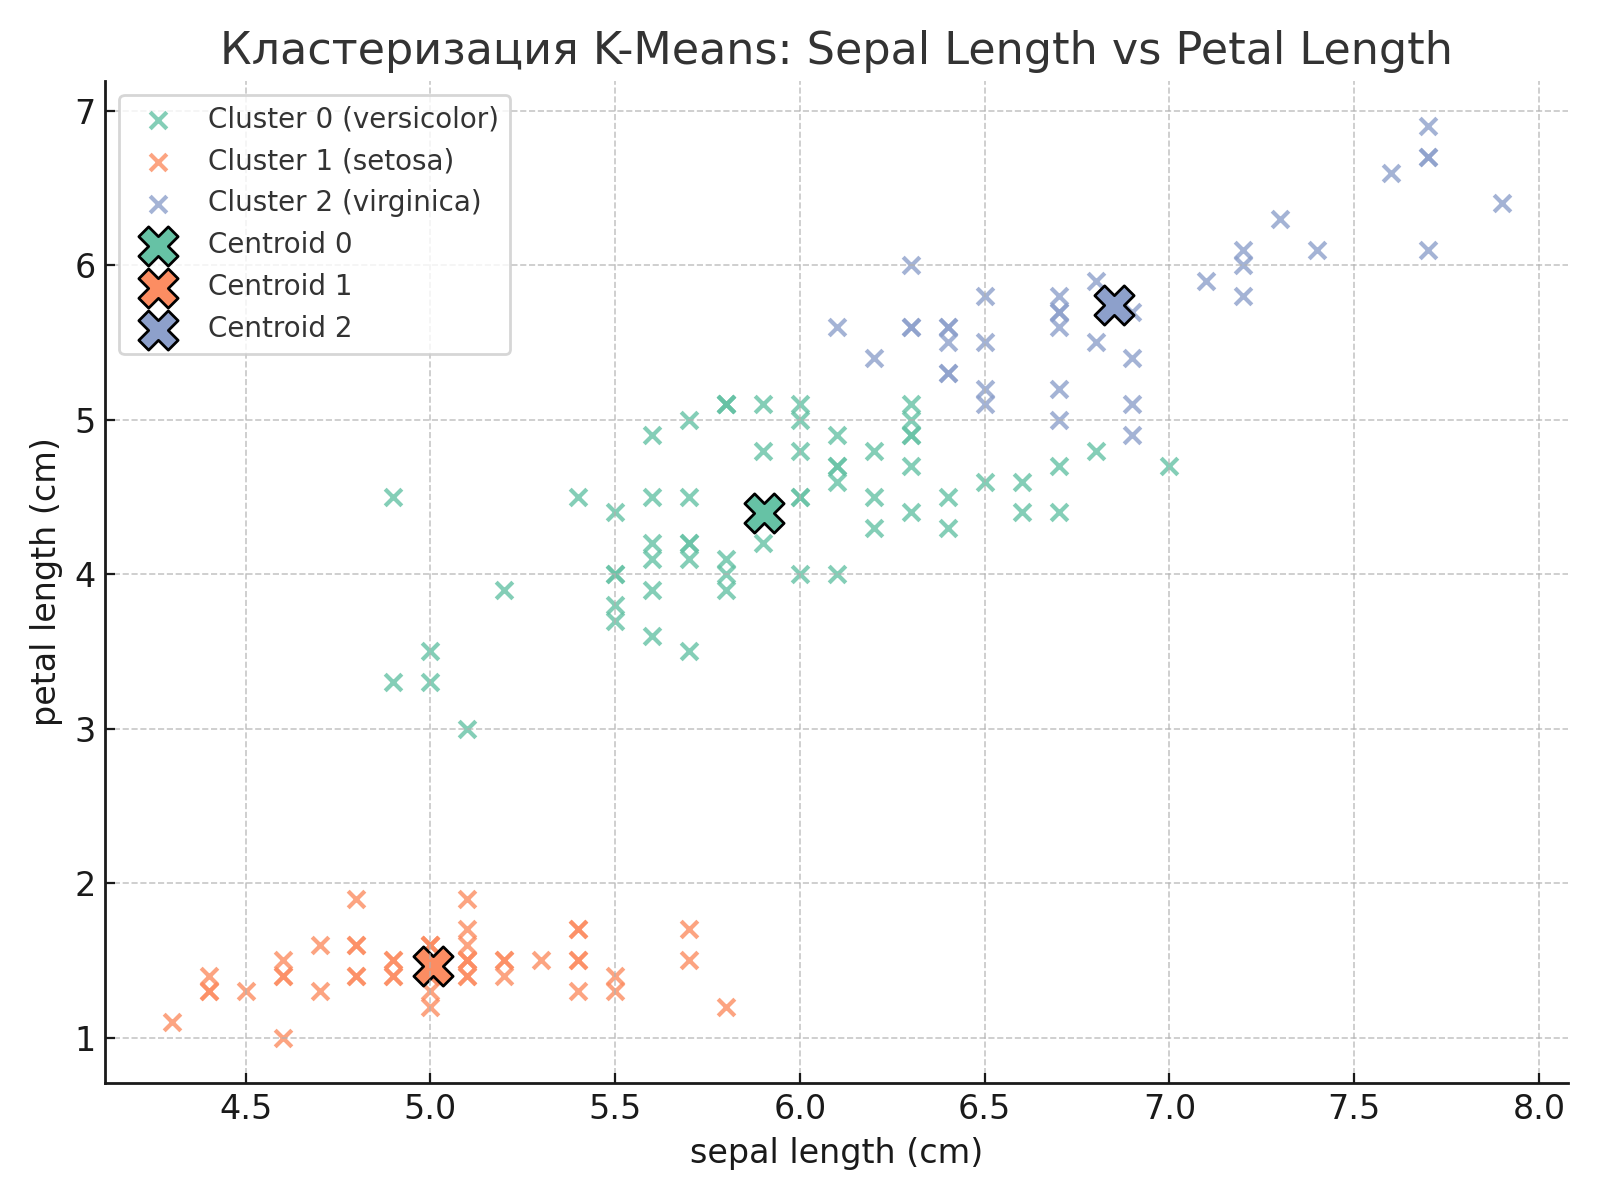
\includegraphics[width=0.8\textwidth]{images/cluster_plot_cb2.png}
  \caption{Кластеризация K–Means: Sepal Length vs Petal Length. Кластеры подписаны с указанием доминирующего вида; центроиды отмечены крупными крестами.}
  \label{fig:kmeans_cb2}
\end{figure}

\paragraph{Выводы.}
\begin{itemize}
  \item \textbf{Cluster 1 (setosa)}: полностью отделён в нижнем левом углу, петаловые признаки минимальны — 100\% точность.
  \item \textbf{Cluster 0 (versicolor)}: средняя область, 48 из 50 экземпляров Versicolor точно отделены (96\%); 14 Virginica попали в этот кластер из–за близости.
  \item \textbf{Cluster 2 (virginica)}: правый верхний угол, 36 из 50 Virginica (72\%), несколько Versicolor «зашли» внутрь.
  \item Итог: лепестковые признаки дают главную разделительную информацию, чашелистики лишь уточняют границы.
\end{itemize}
